\documentclass[a4paper]{article}
\usepackage{amssymb, amsmath}
\usepackage{graphicx}
\begin{document}
\section{Linear Regression}
\subsection{Linear regression and Least Square Solution}
\begin{align*}
Y = X{\boldsymbol \beta} + \epsilon
\end{align*}
Where Y is a n $\times$ 1 matrix, X is a n $\times$ k matrix, beta is k $\times$ 1 vector and $\epsilon$ is nx1 vector with $\epsilon_i$ begin iid with normal distribution.\\
{\bf Assumptions}\\
1. Linear \\
2. X matrix has full rank. In other words, no multicollinearity. \\
2. error term has zero mean $E[\epsilon|X] = 0$\\
3. Homescedasticity or equal variance of $\epsilon$. In other words, no autocorrelation between disturbances.$cov(\epsilon_i, \epsilon_j)=0$.\\
6. Number of obsearvations n must be greater than the number of parameters.\\
{\bf Least Square Solution}\\
The cost function is given by
\begin{align*}
f(\boldsymbol \beta) = ||Y-X\beta||^2 & = (Y-X\beta)^T(Y-X\beta)
                      & = Y^T Y - Y^TX\beta - \beta^TX^TY +\beta^TX^T X \beta
\end{align*}
Since third term are scalar, 
\begin{align*}
 \beta^TX^TY = (\beta^TX^TY)^T = Y^TX\beta 
\end{align*}
\begin{align*}
f(\beta) = Y^T Y - 2Y^TX\beta - \beta^TX^T X \beta
            = Y^T Y - 2(X^TY)^T\beta + \beta^TX^T X \beta
\end{align*}
The first term is a constant and its derivative is zero. \\
{\bf The deriviative of 2nd term}\\
Consider the derivative of $\alpha^T \beta$ with respect to $\beta$.
\begin{align*}
\boldsymbol{\alpha}^T \boldsymbol{\beta} = \Sigma \alpha_i \beta_i \\
\frac{\partial{\boldsymbol{\alpha}^T\boldsymbol{\beta}}}{\partial \beta_i} = \alpha_i\\
\end{align*}
Write the derivative in matrix form
\begin{align*}
\left(  \begin{array} {c}
		\frac{\partial{\boldsymbol{\alpha}^T\boldsymbol{\beta}}}{\partial \beta_1}\\
		\frac{\partial{\boldsymbol{\alpha}^T \boldsymbol{\beta}}}{\partial \beta_2}\\
                  ...\\
		\frac{\partial{\boldsymbol{\alpha}^T \boldsymbol{\beta}}}{\partial \beta_3}\\
		\end{array}
		\right) 
=\left(  \begin{array} {c}
		\alpha_1\\
		\alpha_2\\
                  ...\\
		\alpha_p\\
		\end{array}
		\right) 
\end{align*}
So if we let $\alpha= X^TY$, we have
\begin{align*}
\frac{\partial{2(X^TY)^T\beta}}{\partial \beta} = 2X^TY
\end{align*}
{\bf The derivative of 3rd term}\\
let $A=X^TX$,
\begin{align*}
\beta^TX^T X \beta = \beta^T
\left(  \begin{array} {c}
		\Sigma_i A_{1k}\beta_{k}\\
		 \Sigma_i A_{2k}\beta_{k}\\
                  ...\\
		 \Sigma_k A_{pk}\beta_{k}\\
		\end{array}
		\right) 
 =  \Sigma_j \beta_j (\Sigma_k A_{jk}\beta_k)
\end{align*}
To calculate the derivative of $f(\beta)$, we note there are only 3 cases that the derivative does not vanish\\
1) l = j = k 
\begin{align*}
\frac{f(\boldsymbol \beta)}{\partial \beta_l} 
= 2 A_{ll} \beta_l 
\end{align*}
2) l=j, j $\neq$ k
\begin{align*}
\frac{f(\boldsymbol \beta)}{\partial \beta_l} 
= \Sigma_{k, k\neq l} A_{lk}\beta_{k}\\
\end{align*}
3) l=k, j $\neq$ k
\begin{align*}
\frac{f(\boldsymbol \beta)}{\partial \beta_l} 
= \Sigma_{j, j\neq l} A_{jl}\beta_{j} = \Sigma_{j,  j\neq l} A^T_{lj}\beta{j}
\end{align*}
Therefore
\begin{align*}
\frac{f(\boldsymbol \beta)}{\partial \beta_l}  = A_{ll} \beta_l + \Sigma_{k, k\neq l} A_{lk}\beta_{k} + A_{ll} \beta_l + \Sigma_{j, j \neq l} A^T_{lj}\beta{j} \\
= \Sigma_{k} A_{lk}\beta_{k} + \Sigma_{j} A^T_{lj}\beta{j}
\end{align*}
The first term is the lth row of vector $A\beta = X^TX\beta$, and the 2nd term is the lth row of vector$A^T\beta=X^TX\beta$. So we put the whole derivative in matrix form
\begin{align*}
\frac{f(\boldsymbol \beta)}{\partial {\boldsymbol \beta}} = -2X^TY+2X^TX\beta
\end{align*}
which is a px1 vector with each row corresponding to the derivative with respect to $\beta_i$
letting the derivative equal to zero yields the {\bf normal equation} and the estimation of $\beta$\\
Normal equation
\begin{align*}
(X^TX) \hat \beta = X^TY
\end{align*}
Estimator of $\beta$
\begin{align*}
\hat \beta = (X^TX)^{-1}X^TY
\end{align*}
Using the rule of matrix mutiplication, we can rewrite $X^TX$ as the f
\begin{align*}
X^TX & =
 \left( \begin{array} { c  c  c c } 
                   \sum_{i=1}^N x_{1i}^Tx_{i1} &  \sum_{i=1}^Nx_{1i}^Tx_{i2} & ... & \sum_{i=1}^N x^T_{1i}x_{ik}   \\
                   ... & ... & ... & \\
                   \sum_{i=1}^N x_{ki}^Tx_{i1} &  \sum_{i=1}^Nx_{ki}^Tx_{k2} & ... & \sum_{i=1}^Nx^T_{ki}x_{ik}   \\
           \end{array} \right) \\
    & =  \sum_{i=1}^N
 \left( \begin{array} { c  c  c c } 
                   x_{i1}x_{i1} & x_{i1}x_{i2} & ... & x_{i1}x_{ik}   \\
                   ... & ... & ... & \\
                   x_{ik}x_{i1} & x_{ik}x_{k2} & ... & x_{ik}x_{ik}   \\
           \end{array} \right) \\
      &  =  \sum_{i=1}^N
 \left( \begin{array} { c  } 
                   x_{i1}    \\
                   ...  \\
                   x_{ik}    \\
           \end{array} \right)
 \left( \begin{array} { c c c c } 
                   x_{i1}  & ... &  ... x_{ik}\\ 
           \end{array} \right) \\
     & = \sum_{i=1}^N X_i X_i^T
\end{align*}
where $X_i$ is $K \times 1$ vector, and $X_i X_i^T$ is $K \times K $ matrix.
Similarly,
\begin{align*}
X^TY & = \sum_{i=1}^N X_i y_i
\end{align*}
where $X_i$ is $K \times 1$ vector, $y_i$ is a scalor, and $X_iy_i$ is $K \times 1$ vector.
So the estimator of $\beta$ is
\begin{align*}
\hat \beta = (\sum_{i=1}^N X_i X_i^T)^{-1} (\sum_{i=1}^N X_i y_i)
\end{align*}
{\bf Least Square Estimator for Simple Linear Regression}\\
\begin{align*}
y =  \beta_0 + \beta_1 X + \epsilon\\
\end{align*}
\begin{align*}
	&\left(  \begin{array} {c}
		\beta_{0} \\
		\beta_{1} \\
		\end{array}
		\right) \\
=& (X^TX)^{-1}X^TY \\
=&\left( \left(  \begin{array} {cccc}
		1 & 1 &... &1\\
		x_1 & x_2 &... &x_n \\
		\end{array}
		\right) 
    \left(  \begin{array} {cc}
		1 & x_1 \\
		1 & x_2 \\
                   1 & x_n \\
		\end{array}
		\right) 
\right)^{-1}
\left(  \begin{array} {cccc}
		1 & 1 &... &1\\
		x_1 & x_2 &... &x_n \\
		\end{array}
		\right) 
\left(  \begin{array} {c}
		y_1 \\
		y_2 \\
                  ... \\
                  y_n
		\end{array}
		\right) \\
=& \frac{1}{n\Sigma x^2_i - (\Sigma x_i)^2}
\left(  \begin{array} {cc}
	          \Sigma_i x_i^2 & -\Sigma_i x_i \\
		 -\Sigma_i x_i &n\\
		\end{array}
		\right) 
\left(  \begin{array} {c}
	          \Sigma_i y_i \\
		 -\Sigma x_i y_i\\
		\end{array}
		\right) 
\end{align*}
So
\begin{align} \label{eq:beta0}
\beta_0 & = \frac{\Sigma x_i^2 \Sigma y_i - \Sigma x_i (\Sigma x_i y_i)}{n\Sigma x^2_i - (\Sigma x_i)^2}
\end{align}
\begin{align} \label{eq:beta1} 
\beta_1 & = \frac{n \Sigma x_i y_i -\Sigma x_i \Sigma y_i }{n\Sigma x^2_i - (\Sigma x_i)^2}
\end{align}
$\beta_1$ can also be written using the covariance
\begin{equation} \label{eq:betacovariance}
\beta_1=\frac{\sum_i^n(x_i-\bar x)(y_i-\bar y)}{\sum_i^n(x_i-\bar x)(x_i-\bar x)}
\end{equation}
And it is easy to show 
\begin{align*}
\beta_2 &=\frac{\sum_i^n(x_i-\bar x)(y_i-\bar y)}{\sum_i^n(x_i-\bar x)(x_i-\bar x)}\\
            &=\frac{\sum_i^n(x_iy_i-\bar x y_i -x_i \bar y + \bar x \bar y)}{\sum_i^n(x_i^2 -2\bar x x_i + (\bar x)^2)}\\
	    &=\frac{\sum_i^n x_iy_i-\sum_i^n \bar x y_i -\sum_i^n x_i \bar y + \sum_i^n \bar x \bar y}{\sum_i^n x_i^2 -\sum_i^n 2\bar x x_i + \sum_i^n (\bar x)^2}\\
           &=\frac{\sum_i^n x_iy_i-(\frac{1}{n}\sum_j^n x_j)(\sum_i^n y_i) -(\sum_i^n x_i)(\frac{1}{n}\sum_j^n y_j) + \sum_i^n (\frac{1}{n}\sum_j^n x_i)(\frac{1}{n}\sum_k^n y_i)}{\sum_i^n x_i^2 -\sum_i^n 2(\frac{1}{n}\sum_j^n x_j) x_i + \sum_i^n (\frac{1}{n}\sum_j^n x_j)^2}\\
 &=\frac{\sum_i^n x_iy_i-(\frac{1}{n}\sum_j^n x_j)(\sum_i^n y_i) -(\sum_i^n x_i)(\frac{1}{n}\sum_j^n y_j) + n (\frac{1}{n}\sum_j^n x_i)(\frac{1}{n}\sum_k^n y_k)}{\sum_i^n x_i^2 -\sum_i^n 2(\frac{1}{n}\sum_j^n x_j) x_i + n(\frac{1}{n}\sum_j^n x_j)^2}\\
&=\frac{\sum_i^n x_iy_i-\frac{1}{n}(\sum_i^n x_i)(\sum_j^n y_j) -\frac{1}{n}(\sum_i^n x_i)(\sum_j^n y_j) +  \frac{1}{n}(\sum_j^n x_i)(\sum_k^n y_k)}{\sum_i^n x_i^2 - \frac{2}{n}(\sum_j^n x_j) (\sum_i^nx_i) + \frac{1}{n}(\sum_j^n x_j)^2}\\
&=\frac{\sum_i^n x_iy_i-\frac{1}{n}(\sum_i^n x_i)(\sum_j^n y_j)}{\sum_i^n x_i^2 - \frac{1}{n}(\sum_j^n x_j) (\sum_i^nx_i) }\\
&=\frac{n\sum_i^n x_iy_i-(\sum_i^n x_i)(\sum_j^n y_j)}{n\sum_i^n x_i^2 - (\sum_j^n x_j) (\sum_i^nx_i) }\\
&=\frac{n\sum x_iy_i-(\sum x_i)(\sum_j^n y_j)}{n\sum x_i^2 - (\sum x_i)^2 }\\
\end{align*}
which is the same as Eq.\ref{eq:beta1}.  We can interpret $\beta$ as ratio of the covariance of x and y to the variance of x.
\subsection{Projection matrix}
Given $\hat \beta = (X^TX)^{-1}X^TY$, we have the predictor value of $y=X\beta$ 
\begin{align*}
\hat y = X(X^TX)^{-1}X^T y
\end{align*}
The matrix $P=X(X^TX)^{-1}X^T$ is a projection matrix. It projects the vector of y into the column space of X.\\
{\bf Understand the word projection}\\
Let us understand this first through geometry point of view. Consider a vector on 2 dimensional space, $V_1= (x_1, y_1)^T$, where $x_1$ and $y_1$ are the x and y component, respectively. If we project the vector V into x-line, then apparently we get $V_x= (x_1, 0)^T$, see graph below.

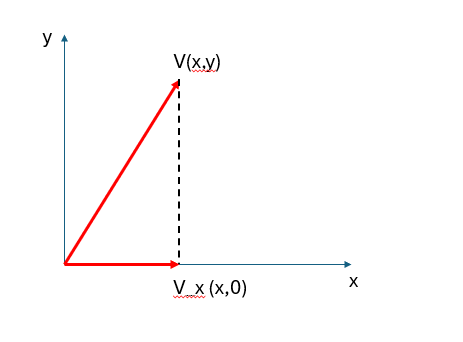
\includegraphics[scale = 1]{project1.png}\\
If we have a vector that is along the x axis
\begin{align*}
X = \left( \begin{array} {c }
              1  \\
              0  \\
            \end{array} \right)\\
\end{align*}
 The projection matrix of a vector into x line is 
\begin{align*}
P_x & = x(x^Tx)^{-1}x^T \\
     & = \left( \begin{array} {c}
              1 \\
              0 \\
            \end{array} \right)
 \left( \begin{array} { c  c } 
                   1 & 0\\
           \end{array} \right) \\
       & =  \left( \begin{array} { c  c } 
                   1 & 0  \\
                   0 & 0  \\
           \end{array} \right)
\end{align*}
Applying this projection matrix to any 2 dimensional vector $V$ gives $(V_x, 0)^T$. So it projects the vector into x line. 
Let us take another example. Imagine $V_1$ is vector if we project $V$ onto the line that has 45 degree angle with x axis. See below.

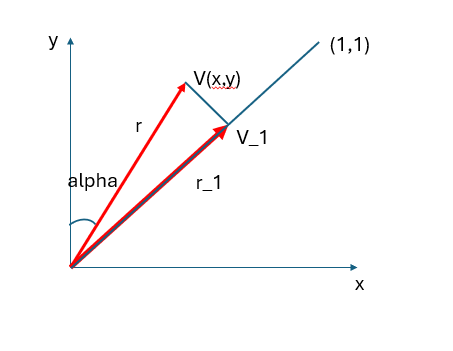
\includegraphics[scale = 1]{project2.png}\\

In order to calculate $V_1$,  we see
\begin{align*}
r_1 = r cos(\pi/4 - alpha) =r( \frac{\sqrt{2}}{2} \frac{y}{r} + \frac{\sqrt{2}}{2} \frac{x}{r}) = \frac{\sqrt 2}{2}y +\frac{\sqrt2}{2} x
\end{align*}
\begin{align*}
V_{1x}=r_1cos(\pi/4)=\frac{x+y}{2}\\
V_{1y}=r_1sin(\pi/4)=\frac{x+y}{2}\\
\end{align*}
After we understand this using geometry point of view, we can workout from algebra point of view. The vector we want to project onto is
\begin{align*}
i = \left( \begin{array} {c }
              1  \\
              1  \\
            \end{array} \right)\\
\end{align*}
The projection matrix of a vector into x line is 
\begin{align*}
P_x & = x(x^Tx)^{-1}x^T \\
     & = \left( \begin{array} {c}
              1 \\
              1 \\
            \end{array} \right)
\left( \left( \begin{array} {c c}
              1 & 1\\
            \end{array} \right) 
          \left( \begin{array} {c }
              1 \\
              1 \\
            \end{array} \right) \right)^{-1}
 \left( \begin{array} { c  c } 
                   1 & 1\\
           \end{array} \right) \\
       & =  \frac{1}{2}\left( \begin{array} { c  c } 
                   1 & 1  \\
                   1 & 1  \\
           \end{array} \right)
\end{align*}
Therefore we easily see
\begin{align*}
V_1 =  \frac{1}{2}\left( \begin{array} { c  c } 
                   1 & 1  \\
                   1 & 1  \\
           \end{array} \right) 
             \left( \begin{array} {c }
              x \\
              y \\
            \end{array} \right)
          = \left( \begin{array} {c }
              \frac{1}{2} (x+y) \\
              \frac{1}{2} (x+y) \\
            \end{array} \right)
\end{align*}
which is the same as what we get based on geometry.
 For n dimensional vector y, if our X matrix has rank of k, then the projection matrix P projects the vector y into k dimensional hyperplane. For example, if we define
\begin{align*}
i_N =   \left( \begin{array} {c }
              1 \\
              1 \\
             ...\\
              1
            \end{array} \right)
\end{align*}
The projection matrix P is
\begin{align*}
P = i \frac{1}{N}i^T
  = \frac{1}{N} \left( \begin{array} { c  c c c } 
                   1 & 1 & ... & 1 \\
                   1 & 1 & ... & 1 \\
                   ... & ... & ... & ... \\
                   1 & 1 & ... & 1 \\
           \end{array} \right) 
\end{align*}
{\bf Projection matrix into null space}\\
If $P$ is a projection matrix, the matrix $I - P$ is also a projection matrix. In linear regression model
\begin{align*}
y &= X\beta +\epsilon\\
P &= X(X^TX)^{-1}X^T\\
\end{align*}
Define residual vector $\hat \epsilon$
\begin{align*}
\hat \epsilon & = (I - P) y = (I - X(X^TX)^{-1}X^T)y\\
\end{align*}
And it is easy to show $\hat e$ and X are orthogonal.
\begin{align*}
X^T \hat \epsilon = X^T (I-P)y =X^T(I - X(X^TX)^{-1}X^T)y = (X^T- X^TX(X^TX)^{-1}X^T)y = 0 y = 0
\end{align*}
For the above example, we define $M = I - \frac{1}{N}i i^T$, and $My$ express the mean deviations of a vector.\\
{\bf Idempotent property of projection matrix\\}
Consider the previous example that we project a vector V onto x axis, how about we do this projection twice, we would end up the same vector $V_x$. Using a little matrix algebra, it is easy to prove that for any project matrix P, we have $PP=P$.  
\subsection{Partitioned Regression and  Regression}
\begin{align*}
y = X \boldsymbol \beta + \epsilon = X_1 \beta_1 + X_2 \beta_2 + \epsilon
\end{align*}
The normal equation is
\begin{align*}
 \left( \begin{array} { c  c } 
                   X_1^TX_1 & X_1^TX_2  \\
                   X_2^TX_1 & X_2^TX_2   \\
           \end{array} \right)
 \left( \begin{array} { c  } 
                   \hat \beta_1   \\
                   \hat \beta_2   \\
           \end{array} \right) =
\left( \begin{array} { c  } 
                   X_1^T y   \\
                   X_2^T y   \\
           \end{array} \right)
\end{align*}
If X1 and X2 are orthogonal, namely, $X_1^T X_2=0$, then 
\begin{align*}
\boldsymbol {\hat  \beta_1} = (X_1^T X_1)^{-1} X_1^Ty\\
\boldsymbol {\hat  \beta_2} = (X_2^T X_2)^{-1} X_2^Ty
\end{align*}
If X1 and X2 are not orthogonal, we can solve for $\beta_2$ in the above normal equation set and get $\beta_2$
\begin{align*}
\hat \beta_2 & = [X_2^T(I-X_1(X_1^TX_1)^{-1}X_1^T)X_2]^{-1}[X_2(I-X_1(X_1^TX_1)^{-1}X_1^T)y]\\
& = (X_2^T M_1X_2)^{-1}(X_2^T  M_1y) \\
\end{align*}
Given the fact that $M_1$ is symmetrical and idempotent, we can rewrite the above expression
\begin{align}
\hat \beta_2  & = (X_2^T M_1 M_1X_2)^{-1}(X_2^T M_1 M_1y)  \notag \\
&= (X_2^T M_1^T M_1X_2)^{-1}(X_2^TM_1^T M_1y) \notag \\
& = ((M_1 X_2)^T  M_1X_2)^{-1}((M_1 X_2)^T M_1y)  \label{eq:partial} 
\end{align}
The above uses the property that $M_1^T=M_1$ and $M_1 M_1 = M_1$\\
The $\hat \beta_2$ is also the solution of 
\begin{align*}
 M_1 Y = M_1 X_2 \beta_2 + \epsilon
\end{align*}
where $M_1 y$ is the residual of y regressed on $X_1$ and $M_1 X_2$ is the residual of $X_2$ regressed on $X_1$.
For example, in simple linear regression
\begin{align*}
Y= \beta_0 + x\beta_1
\end{align*}
Where $X_1=1_N$, so its projection matrix is $i\frac{1}{N}i^T$, and the corresponding M matrix is $I - \frac{1}{N}ii^T$.
We tries to calculate $\beta$ using partition regression. 
\begin{align*}
MY = (I-\frac{1}{N}ii^T)Y = Y-\bar Y
MX = (I-\frac{1}{N}ii^T)Y = X-\bar X
\end{align*}
Then
\begin{align}
\beta_1 = ((MX)^T(MX))^{-1}((MX)^T(MY))  = \frac{\sum_i^N(x_i - \bar x)(y_i - \bar y)}{\sum_i^N(x_i-\bar x)^2} \label{eq:beta_partition}
\end{align}
which is the same as Eq.\ref{eq:betacovariance}
\subsection{Variance componet identity}
If we define our mean projection matrix P 
\begin{align*}
P = i \frac{1}{N}i^T
\end{align*}
and silimarly we define mean deviation project matrix 
\begin{align*}
M= I-P = i\frac{1}{N}i^T
\end{align*}
We have
\begin{align*}
y= \hat y + \hat \epsilon = X\hat \beta + \hat \epsilon
\end{align*}
Multiplying M matrix on the left, we have
\begin{align*}
My= MX\hat \beta + M \hat \epsilon = MX\hat \beta +\hat \epsilon
\end{align*}
\begin{align*}
(My)^2 &= (MX\hat \beta + \hat \epsilon)^T(MX\hat \beta +  \hat \epsilon) \\
&=(\beta^T X^T M^T + \hat \epsilon^T )(MX\hat \beta + \hat \epsilon) \\
&=(MX\hat \beta)^2 + \beta^T X^T M^T \hat \epsilon+ (\beta^T X^T M^T \hat \epsilon)^T  + (\hat \epsilon)^2\\
\end{align*}
The 2nd and 3rd terms are zero because that 1)$\hat \epsilon$ has zero mean, so $M^T\hat \epsilon = M \hat \epsilon = \hat \epsilon$ and 2) $X^T\hat \epsilon = 0$, so
\begin{align*}
(My)^2 &=(MX\hat \beta)^2 + (\hat \epsilon)^2\\
\end{align*}
Rewriting the above equation using summation, we have
\begin{align*}
\sum_i (y_i - \bar y)^2 =\sum_i^N (\bar y_i - \bar {\hat y})^2 + \sum_i(y_i-\hat y)^2
\end{align*}
Define
\begin{align*}
SST & = \sum_i (y_i - \bar y)^2 \\
SSR & = \sum_i (\bar y_i - \bar {\hat y})^2 \\
SSE & = \sum_i(y_i-\hat y)^2\\
\end{align*}
SSE can also be written as
\begin{align*}
SSE & = SST- SSR\\
      & = SST - (MX\hat \beta)^2\\
      & = SST - ((MX)((MX)^T(MX))^{-1}(MX)^T(MY))^2 
\end{align*}
Let $U = MX$, and$V= MY$ then
\begin{align*}
SSE & = SST - (Z(Z^TZ)^{-1}Z^T)^2 \\
      &  = SST - (U(U^TU)^{-1}U^TV)^T (U(U^TU)^{-1}U^TV) \\
      &  = SST - V^TU(U^TU)^{-1}U^TU(U^TU)^{-1}U^TV\\
      &  = SST - V^TU(U^TU)^{-1}U^TV\\
      &  = SST - (MY)^T(MX)((MX)^T(MX))^{-1}(MX)^T(MY)\\
\end{align*}
Define
\begin{align*}
S_{xx} &= (MX)^T(MX)  = \sum_{i}^N (x_i - \bar x)^2\\
S_{xy} &= (MX)^T(MY) = \sum_{i}^N (x_i - \bar x)(y_i -\bar y)\\
\end{align*}
So
\begin{align*}
SSE = SST - S_{xy}^T S_{xx}^{-1} S_{xy}
\end{align*}

Then we have
\begin{align*}
SST = SSR + SSE
\end{align*}
\subsection{Variance of $\hat \beta$ and $\sigma^2$ estimation}
\begin{align*}
Var(\hat \beta)
=Var((X^TX)^{-1}X^T \epsilon)
=(X^TX)^{-1}X^T Var( \epsilon) ((X^TX)^{-1}X^T)^T\\
=\sigma^2 (X^TX)^{-1}X^T  X (X^TX)^{-1}
=\sigma^2 (X^TX)^{-1}
\end{align*}
The above derivation use the fact that $\epsilon$ has a normal distribution with mean 0 and variance $\sigma^2$.
For simple linear regression
\begin{align*}
Var(\hat \beta)
=\frac{\sigma^2}{n\Sigma x_i^2 - (\Sigma x_i)^2} \left(  \begin{array} {cc}
	          \Sigma_i x_i^2 & -\Sigma_i x_i \\
		 -\Sigma_i x_i &n\\
		\end{array}
		\right) 
\end{align*}
\begin{align*}
Var(\hat \beta_0) =\frac{\Sigma x_i^2 \sigma^2}{n\Sigma x_i^2 - (\Sigma x_i)^2} 
\end{align*}
\begin{align*}
Var(\hat \beta_1) =\frac{n \sigma^2}{n\Sigma x_i^2 - (\Sigma x_i)^2} 
\end{align*}
Try
\begin{align*}
\Sigma (x_i- \bar x)^2 = \Sigma(x_i^2 - 2 \bar x x_i+ \bar x^2)
= \Sigma_i(x_i^2 - 2 (\Sigma_j \frac{x_j}{n}) x_i + \frac{ (\Sigma_j x_j)^2} {n^2})\\
=\Sigma_ix_i^2 - \frac{2}{n} (\Sigma_i x_i)^2 + \frac{ (\Sigma_i x_i)^2} {n}
= \Sigma_i x^2_i - \frac{1}{n} (\Sigma x_i)^2
\end{align*}
So
\begin{align*}
Var(\hat \beta_0) =\frac{\Sigma x_i^2 \sigma^2}{n\Sigma (x_i- \bar x)^2 } 
\end{align*}
\begin{align*}
Var(\hat \beta_1) =\frac{n \sigma^2}{n\Sigma (x_i- \bar x)^2} = \frac{\sigma^2}{\Sigma (x_i- \bar x)^2}
\end{align*}
\begin{align*}
SSE
&=\Sigma_i (y-\hat y_i)^2 \\
& = (Y-X\beta)^T(Y-X\beta) \\
& = (Y-X(X^TX)^{-1}X^TY)^T(Y-X(XTX)-1X^TY) \\
& = (Y-PY)^T(Y-PY) \\
& = Y^T(1-P)^T(1-P)Y = Y^T(1-P)Y \\
& = (X\beta + \epsilon) ^T (1-P)(X\beta+\epsilon) \\
& = \beta^T X^T (1-P)X\beta + 2\beta^T X^T X^T(I-P)\epsilon 
   + \epsilon^T(I-H)\epsilon 
\end{align*}
\begin{align*}
E[SSE] = E[\epsilon^T(I-P)\epsilon] = E[\epsilon^T \epsilon] trace(I-H)
          = \sigma^2(n-k)\\
\end{align*}
We obtain the unbiased estimator of $\sigma^2$\\
\begin{align*}
\hat \sigma^2 = \frac{SSE}{n-k}
\end{align*}
Therefore the estimator of variance of $\beta$
\begin{align*}
\hat Var(\hat \beta_i) = \hat \sigma^2(X^TX)^{-1}_{ii}
\end{align*}
and the stanard error of $\beta_i$ is
\begin{align*}
SE(\hat \beta_i) = \sqrt{ \hat \sigma^2(X^TX)^{-1}_{ii}}
\end{align*}
\section{Properties of Least Square Estimators}
When we have a estimator, we need to evaluate how good our estimator is? A few questions we can ask is 1): how far is the value of our estimator away from the true value, even in the ideal case when the sample size is inifinite? 2) when 1) is true, with finite sample size, does the value of our estimator approach to the true value as the sample size increase? In other words, does the estimator converge to the true value as sample size goes to inifinity? 3) when 1) and 2) is true, as the sample size increase, how fast does our estimator converges to true value? 4) with 1) 2) and 3), what is the asymptotic distribution of the estimator? If the distribution is normal, it can be used to do interval estimation such as confidence interval. The 1st question defines unbiasness, the 2nd one defines consistency, and the 3rd one defines efficiency.\\ 
\subsection{Unbiasness}
{\bf Unbiased}\\
\begin{align*}
\hat \beta & = (X^T X)^{-1}X^TY\\
               & = (X^T X)^{-1}X^T(X \beta + \epsilon)\\
               & = (X^T X)^{-1}X^T X \beta   + (X^T X)^{-1}X^T \epsilon\\
               & = \beta +  (X^T X)^{-1}X^T \epsilon\\
\end{align*}
Then the expectation of $\hat \beta$ condition on X is
\begin{align*}
E[{\hat \beta|X}] = \beta + (X^TX)^{-1} X^T E(\epsilon|X)\\t
\end{align*}
The last term is zero by assuption of linear regression. So 
\begin{align*}
E[\hat \beta] = \beta
\end{align*}
The expectation of the estimator is the same as true value, this is called {\bf unbiased}. \\
{\bf Bias due to omission of relevant variables}\\
Suppose we have a model
\begin{align*}
y = X_1 \beta_1 + X_2 \beta_2 + \epsilon
\end{align*}
If we regression y on $X_1$ only, our estimator is
\begin{align*}
\hat \beta_1 = (X_1^T X_1)^{-1} X_1^T y = \beta_1 + (X_1^TX_1)^{-1}X_1^TX_2\beta_2 + (X_1^TX_1)^{-1}X_1^T\epsilon
\end{align*}
On the second term, we see unless 1)$X_1$ and $X_2$ are orthogonal, or 2)$\beta_2$ =0,  $\beta_1$ is biased.\\
\subsection{Consistency}
The unbiasness gives us a metric of measuring how good our esitimator is, from population perspetive. In reality, as our sample size is finite, we need ask ourselves does our estimator converges to true value when sample size is sufficiently large. We know
\begin{align*}
\hat \beta = \beta + (X^TX)^{-1}X^T\epsilon
\end{align*}

\begin{align*}
\hat \beta &= \beta + ({X^TX})^{-1} {X^T \epsilon} \\
               &= \beta + ( \Sigma_{i=1}^N X_i X_i^T)^{-1} X^T \epsilon \\
               &= \beta + ( \Sigma_{i=1}^N  \frac{1}{N}{X_iX_i^T})^{-1}(\frac{X^T \epsilon}{N})
\end{align*}
To show $\hat \beta$ converges to $\beta$, we need to show two things:\\
(1)$\frac{1}{n}\sum_i{X_iX_i^T}$  converges to Q in probability when N is large. Also the inverse of Q exists.\\
(2)$\frac{X^T \epsilon}{N}$ converges to zero in probability when N is large.\\
For (1), we write
\begin{align*}
Q^{(n)} = \frac{1}{n}\sum_i{X_iX_i^T}
\end{align*}
which is a $K \times K$ matrix. Its element $Q_{kl}$ is
\begin{align*}
Q^{(n)}_{kl} = \frac{1}{n} \sum_i x_{ik} x_{il}
\end{align*}
Based on Law of large numbers, $Q^{n}_{kl}$ converges to its expectation value $E[x_{ik}x_{il}]$. Let
\begin{align*}
E[x_{ik}x_{il}]=Q_{kl}
\end{align*}
So each element of $Q^{(n)}$ converges $Q_{kl}$. Therefore, $Q^{(n)}$ converges to Q. To show the inverse of Q exists, we can show Q is a symmetric positive definite matrix. For any k dimenional vector v, we have
\begin{align*}
v^TQv = E[v^T x_i x_i^T v]
\end{align*}
Since $v^T x_i = \sum_k v_k x_{ik} = x_i^T v$ which is a scalar, so
\begin{align*}
v^TQv = E[v^T x_i x_i^T v] = E[(v^T x_i)^2]
\end{align*} 
if for any i, $x_{ik}$ are linear independent, in other words, no multicollinearity. Then $v^T x_{i} =\sum_k v_k x_{ik} \neq 0$ and $(v^T x_i)^2>0$. Therefore Q is SPD matrix and its inverse exists.
\begin{align*}
&\frac{X^T \epsilon}{N}\\ 
 =& \left(\begin{array} {c}
       \frac{1}{N}\Sigma_{1}^{N}x_{i1}\epsilon_i \\
       \frac{1}{N}\Sigma_{1}^{N}x_{i2}\epsilon_i \\
       \frac{1}{N}\Sigma_{1}^{N}x_{i3}\epsilon_i \\
       ... \\ 
      \frac{1}{N}\Sigma_{1}^{N}x_{ik}\epsilon_i\\
     \end{array} \right)\\
=& \frac{1}{N}\Sigma_{i=1}^{N} X_i\epsilon_i = \bar w\\
\end{align*}
Where $\bar w$ is a k $\times$ 1 vector. To see the asymptotical behavior of $w$, we consider its mean and asymptotical varance. The mean is
\begin{align*}
E[w_i]=E_X[E[w_i|x_i]] = E_X[X_iE[\epsilon|X_i]] = 0
\end{align*}
\begin{align*}
Var[\bar w]=E[Var[\bar w|X]]+Var[E[\bar w|X]] = E[Var[\bar w|X]]+0 = E[Var[\bar w|X]]
\end{align*}
\begin{align*}
Var[\bar w|X] = E[\bar w \bar w^T|X]=\frac{1}{n}X^TE[\epsilon \epsilon^T]X\frac{1}{n} = \frac{\sigma^2}{n}\frac{X^T X}{n}
\end{align*}
\begin{align*}
E[Var[\bar w|X]] = \frac{\sigma^2}{n}E(\frac{X^TX}{n})
\end{align*}
We have shown that $X^TX = \sum_i x_i x_i^T$, so 
\begin{align*}
\frac{X^TX}{n} = \frac{1}{n}\sum_i x_i x_i^T 
\end{align*}

When $\frac{X^TX}{n}$ converges to Q, 
\begin{align*}
E[Var[\bar w|X]] = 0
\end{align*} 
So $\bar w$ converges to $\boldsymbol 0(k \times 1)$ vector. Then when N is sufficiently large, $\hat \beta$ converges to $\beta$. This is the proof of consistency.\\
There are certain conditions in which the estimators become inconsitent.\\
1) X is not full rank, or X has multicollinearity
2) $cov[X, \epsilon] \neq 0$
\subsection{Efficiency}
The least equare estimator has the smallest varaince, and this can be proved by Gauss-Markov theorem. 
\subsection{Multicollinearity}
Suppose we have a regression model that contains two parameters
\begin{align*}
y = \beta_0 + X_1\beta_1 + X_2 \beta_2
\end{align*}
From above, we know variance of ${\bf \hat \beta}$ is
\begin{align*}
Var(\hat \beta) = \frac{\sigma^2}{(X^TX)^{-1}}
\end{align*}
When X only contains 2 variables, $X=(X_1, X_2)$
\begin{align*}
Var(\hat \beta_1) = \sigma^2 \frac{S_{22}}{S_{11}S_{22}-S_{12}^2} = \frac{1}{S_{11}(1-\frac{S^2_{12}}{S_{11}S_{22}})}= \frac{1}{S_{11}(1-r_{12}^2)} \\
Var(\hat \beta_2) = \sigma^2 \frac{S_{11}}{S_{11}S_{22}-S_{12}^2} = \frac{1}{S_{22}(1-\frac{S^2_{12}}{S_{11}S_{22}})}= \frac{1}{S_{22}(1-r_{12}^2)} \\
\end{align*}
Where
\begin{align*}
S_{11} & =\Sigma(x_{1i}-\hat x_1)^2\\
S_{22} & =\Sigma(x_{2i}-\hat x_2)^2\\
S_{12} & =\Sigma(x_{1i}-\hat x_1)(x_{2i}-\hat x_2)\\
r_{12} & = \frac{S_{12}}{\sqrt{S_{11}S_{22}}}\\
\end{align*}
$r_{12}$ is the correlation coefficient. In extreme case, when $X_1$ and $X_2$ are perfectly correlated, the variance becomes infinite.\\
\section{Model Testing}
{\bf Lagrange Multiplier(LM) test}\\
Suppose we have two models, one is restriced, the other is unrestricted:
Restricted(R): $y = X_1 \beta_1 + \epsilon$\\
Unrestricted (U): $y = X_1 \beta_1 + X_2 \beta_2 + \epsilon$\\
Given the unrestricted model, the likehood function is 
\begin{align*}
L(\beta_1, \beta_2, \sigma^2) = \frac{1}{(2\pi \sigma^2)^{n/2}}exp(-\frac{1}{2\sigma^2}(y-X_1\beta_1-X_2\beta_2)^T(y-X_1\beta_1-X_2\beta_2))
\end{align*}
\begin{align*}
S_2 = \frac{\partial L}{\partial \beta_2} =\frac{1}{\sigma^2}X_2^T(y - X_1\beta_1-X_2\beta_2)
\end{align*}
When $\beta_2=0$, define
\begin{align*}
M_1 = I - X_1(X^T_1X_1)^{-1}X^T_1
\end{align*}
and $M_1X_1=0$.
\begin{align*}
S_2 =\frac{1}{\sigma^2}X_2^T(y-X\hat \beta_1)=\frac{1}{\sigma^2}X_2^TM_1y = \frac{1}{\sigma^2}X_2^TM_1(X_1 \beta_1 + \epsilon) = \frac{1}{\sigma^2}X_2^TM_1 \epsilon
\end{align*}
The last equal sign uses the fact $M_1X_1 = 0$.
\begin{align*}
 Var(X_2^TM_1 \epsilon) & = Var(X_2^TM_1 \epsilon) \\
             & =  X_2^TM_1Var(\epsilon)(X_2^TM_1)^T \\
             & =  X_2^TM_1 M_1^T X_2Var(\epsilon) \\
             & = \sigma^2  X_2^TM_1X_2 \\
\end{align*}
Define
\begin{align*}
V =  X_2^TM_1X_2
\end{align*}
Then
\begin{align*}
Var(X_2^T M_1 \epsilon) = \sigma^2V
\end{align*}
So $X_2^TM_1\epsilon$ follows normal distribution with mean 0 and variance $\sigma^2X_2^TM_1X_2$. Define
\begin{align*}
Z=\frac{X_2^TM_1\epsilon}{\sqrt{\sigma^2X_2^TM_1X_2}} = \frac{S_2}{\sqrt{\sigma^2V}}
\end{align*}
then Z follows standard normal distribution. The {\bf Lagrange Multiplier (LM) test} is defined
\begin{align*}
LM =  Z^2  = \frac{(X_2^TM_1\epsilon)^2}{\sigma^2X_2^TM_1X_2} = \frac{S_2^2}{\sigma^2 V}
\end{align*}
which follows $\chi^2$ distribution with degree of freedom 1.\\
{\bf F test}\\
We define
\begin{align*}
SSE_U = ||y -X_1\hat\beta_1 - X_2\hat\beta_2||^2\\
SSE_R = ||y -X_1\hat\beta_1 ||^2
\end{align*}
F test is defined as
\begin{align*}
F = \frac{\frac{Extra \hspace{1mm} expalined \hspace{1mm} variation}{Degree \hspace{1mm} of \hspace{1mm} Freedom}}{\frac{Remaining \hspace{1mm}  unexplained \hspace{1mm} variation}{Degree \hspace{1mm} of \hspace{1mm} Freedom}} = \frac{SSE_R - SSE_U}{\frac{SSE_U}{n-1}}
\end{align*}
Let $X=(X_1, X_2)$, and we define two projection matrices
\begin{align*}
P_U = X(X^TX)^{-1}X^T\\
P_R = X_1(X_1^TX_1)^{-1}X_1^T
\end{align*}
\begin{align*}
SSR_R-SSR_U=y^TP_Ry-y^TP_Uy = y^T(P_R-P_U)y
\end{align*}
recall
\begin{align*}
\hat \beta_2 = (X_2^T M_1 X_2)^{-1}X_2^TM_1 y
\end{align*}
The corresponding projection matrix is
\begin{align*}
M_1X_2 (X_2^T M_1 X_2)^{-1}X_2^TM_1
\end{align*}
The $SSR_R$ - $SSR_U$ is the additional variance explained by $X_2$ after removing the linear space of $X_1$ on $X_2$.  This means the projection matrix corresponding to $\beta_2$ is $P_U$ - $P_R$. So we can get $P_U$ - $P_R$ using the interpretation of projection matrix instead solving for the projection matrix itself.
\begin{align*}
P_U-P_R & =M_1X_2(X_2^TM_1X_2)^{-1}X_2^TM_1\\
\end{align*}
The extra expained sum of squares by the unrestricted model is
\begin{align*}
SSR_R-SSR_U & = y^T(P_R-P_U)y = (X_2^TM_1y)^T(X_2^TM_1X_2)^{-1}X_2^TM_1y
\end{align*}
with 1 degree of freedom as $X_2$ only contains 1 parameter.
\begin{align*}
F = \frac{SSR_R - SSR_U}{\frac{SSR_U}{n-k}} = \frac{(X_2M_1y)^T(X_2^TM_1y)}{\hat \sigma^2 (X_2^TM_1X_2)} =LM
\end{align*}
We see that F test and LM test are equivalent.\\
{\bf Wald Test}\\
Recall the estimator for $\beta_2$ in Eq.\ref{eq:partial},
\begin{align*}
\hat \beta_2  =  (X_2^T  M_1X_2)^{-1}(X_2^T M_1y)  
\end{align*}
Substitue
\begin{align*}
y=X_1\beta_1+X_2\beta_2+\epsilon
\end{align*}
we get
\begin{align*}
\hat \beta_2 =  (X_2^T  M_1X_2)^{-1}(X_2^T M_1\epsilon)  
\end{align*}
Since $\epsilon ~ N(0, \sigma^2I)$, we obtain
\begin{align*}
\beta_2 \sim N(0, \sigma^2(X_2^TM_1X_2)^{-1})
\end{align*}
Thus, scaling by $1/\sigma^2$, we arrive at
\begin{align*}
\frac{1}{\sigma^2}X_2^T M_1\epsilon \sim N(0,X_2^T M_1 X_2 )
\end{align*}
Construct Wald test W
\begin{align*}
W = \frac{\hat \beta_2}{\sqrt{\hat Var(\hat \beta_2)}}
\end{align*}
W follows t distribution. We now show W test is equivalent to LM test. Consider $W^2$
\begin{align*}
W^2 & =\hat \beta^T (Var(\hat \beta))^{-1} \hat \beta = \frac{1}{\sigma^2}\hat \beta^T V \hat \beta = \frac{1}{\sigma^2} (V^{-1}S_2)^T V V^{-1} S_2 =\frac{1}{\sigma^2} S_2^T V^{-1}VV^{-1}S_2 \\ &=  \frac{1}{\sigma^2}S_2^T V^{-1}S_2\\
       &= LM
\end{align*}
\section{Panel Data Model}
We can view panel data as a "two dimensional" data set in which the sample does not only come from different individuals, but also same individual across different time point.  We can write the regression model as
\begin{align*}
y_{it} = \alpha_{it} + \sum_k x_{itk} \beta_{itk} + u_{it}
\end{align*}
where $1<i<N$, $1<t<T$, and $1<k<K$. The equation has total sample size of $NT$ with total number of parameter $NT(K+1)$, therefore it is not estimable. So we will make the following few assumptions\\
\begin{tabular}{c |c | c | c | c}
&$\alpha_{it} = \alpha_{is}$ & $\alpha_{it} = \alpha_{jt}$ & $\beta_{it} = \beta_{is}$ & $\beta_{itk} = \beta_{jtk}$\\ 
\hline
Pooled&yes&yes&yes&yes\\
Fixed Effect&yes&no&yes&yes\\
Unrestricted&yes&no&yes&no\\
\end{tabular}
\subsection{The unrestriced model}
\begin{align*}
y_{it}=\alpha_i + \sum_k x_{itk}\beta_{ik} + u_{it}
\end{align*}
The above equation can be written in matrix form:\\
for $i = 1$,
\begin{align*}
 \left( \begin{array} { c  } 
                   y_{11}  \\
                   y_{12}  \\
                   ... \\
                   y_{1T} \\
           \end{array} \right)
       = \left( \begin{array} { c c c c c } 
                 1 &  x_{111} & x_{112} & ... & x_{11K} \\
                 1 &  x_{121} & x_{122} & ... & x_{12K}\\
                 1 &  ... & ... & ...&...\\
                 1 &  x_{1T1} & x_{1T2} & ... &x_{1TK}\\
           \end{array} \right)
            \left( \begin{array} { c } 
                   \alpha_1 \\
                   \beta_{11}  \\
                   \beta_{12}  \\
                   ... \\
                   \beta_{1K} \\
           \end{array} \right)
               +
            \left( \begin{array} { c  } 
                   u_{11}  \\
                   u_{12}  \\
                   ... \\
                   u_{1T} \\
           \end{array} \right)
\end{align*}
which we can also write as
for $i = 2$,
\begin{align*}
 \left( \begin{array} { c  } 
                   y_{21}  \\
                   y_{22}  \\
                   ... \\
                   y_{2T} \\
           \end{array} \right)
       = \left( \begin{array} { c c c c c } 
                 1 &  x_{211} & x_{212} & ... & x_{21K} \\
                 1 &  x_{221} & x_{222} & ... & x_{22K}\\
                 1 &  ... & ... & ...&...\\
                 1 &  x_{2T1} & x_{2T2} & ... &x_{2TK}\\
           \end{array} \right)
            \left( \begin{array} { c } 
                   \alpha_2 \\
                   \beta_{21}  \\
                   \beta_{22}  \\
                   ... \\
                   \beta_{2K} \\
           \end{array} \right)
               +
            \left( \begin{array} { c  } 
                   u_{21}  \\
                   u_{22}  \\
                   ... \\
                   u_{2T} \\
           \end{array} \right)
\end{align*}
So for each i, we can write
\begin{align*}
Y_i = 1_T \alpha_i+ X_i \beta_i + U_i
\end{align*}
where $Y_i = (y_{i1}, y_{i2}, ...,y_{iT})^T$, $1_T$ is a one vector of length T, $X_i$ is $K \times T $ matrix, $\beta_i = (\beta_{i1}, \beta_{i2}, ...,\beta_{iK})^T$, and $U_i = (u_{i1}, u_{i2}, ...,u_{iT})^T$.

If we consolidate equation set for all the value of i
\begin{align*}
 \left( \begin{array} { c  } 
                   Y_{1}  \\
                   Y_{2}  \\
                   ... \\
                   Y_{N} \\
           \end{array} \right)
       = \left( \begin{array} { c c c c c } 
                 1_{T} & 0 & 0 & ... & 0\\
                 0 & 1_{T} & 0 & ...& 0\\
                 0 & 0 & 1_{T} & ...& 0\\
                 0 &  0 & 0 & ... &1_{NT}\\
           \end{array} \right)
            \left( \begin{array} { c } 
                   \alpha_{1}  \\
                   \alpha_{2}  \\
                   ... \\
                   \alpha_{N} \\
           \end{array} \right) +
\left( \begin{array} { c c c c c } 
                 X_{1} & 0 & 0 & ... & 0\\
                 0 & X_{2} & 0 & ...& 0\\
                 0 & 0 & X_{3} & ...& 0\\
                 0 &  0 & 0 & ... &X_{N}\\
           \end{array} \right)
            \left( \begin{array} { c } 
                   \beta_{1}  \\
                   \beta_{2}  \\
                   ... \\
                   \beta_{N} \\
           \end{array} \right)
               +
            \left( \begin{array} { c  } 
                   U_{1}  \\
                   U_{2}  \\
                   ... \\
                   U_{N} \\
           \end{array} \right)
\end{align*}
To solve for $\beta_i$, we can use the strategy of partition regression. $\beta_i$ is the solution of the the regression
\begin{align*}
MY_i= MX_i\beta + U
\end{align*}
where 
\begin{align*}
M & = I -\frac{1}{T}1_T 1_T^{'} \\
MY_i & = y_{it}-\bar y_{i.} \\
MX_i & = x_{it}-\bar x_{i.} \\
\end{align*}
Here to avoid duplicate notation, we denote the transposed matrix using $'$. The estimate of $\beta$ is
\begin{align*}
\hat \beta_i = ((MX_i)^T(MX_i))^{-1}((MX_i)^T(MY_i))=  W_{xx,i}^{-1}W_{xy,i}
\end{align*}
where 
\begin{align*}
W_{xy,i} &= \sum_t^T(x_{it}-\bar x_{i.})(y_{it}-\bar y_{i.}) \\
W_{xx,i} &= \sum_t^T(x_{it}-\bar x_{i.})(x_{it}-\bar x_{i.})^T
\end{align*}
\subsection{The pooled model}
\begin{align*}
y_{it}=\alpha + \sum_k x_{itk}\beta_{k} + u_{it}
\end{align*}
The above equation can be written in matrix form:\\
for $i = 1$,
\begin{align*}
 \left( \begin{array} { c  } 
                   y_{11}  \\
                   y_{12}  \\
                   ... \\
                   y_{1T} \\
                   y_{21} \\
                   y_{22} \\
                   ... \\
                   y_{2T}\\
                   ...\\
                   y_{NT}\\
           \end{array} \right)
       = \left( \begin{array} { c c c c c } 
                 1 &  x_{111} & x_{112} & ... & x_{11K} \\
                 1 &  x_{121} & x_{122} & ... & x_{12K}\\
                 1 &  ... & ... & ...&...\\
                 1 &  x_{1T1} & x_{1T2} & ... &x_{1TK}\\
           	 1 &  x_{211} & x_{212} & ... & x_{21K} \\
                 1 &  x_{221} & x_{222} & ... & x_{22K}\\
                 1 &  ... & ... & ...&...\\
                 1 &  x_{2T1} & x_{2T2} & ... &x_{2TK}\\
                 1 &  ... & ... & ...&...\\
                 1 &  x_{NT1} & x_{NT2} & ... &x_{NTK}\\
           \end{array} \right)
            \left( \begin{array} { c } 
                   \alpha \\
                   \beta_{1}  \\
                   \beta_{2}  \\
                   ... \\
                   \beta_{K} \\
           \end{array} \right)
               +
            \left( \begin{array} { c  } 
                   u_{11}  \\
                   u_{12}  \\
                   ... \\
                   u_{1T} \\
   		   u_{21}  \\
                   u_{22}  \\
                   ... \\
                   u_{2T} \\
                   ...\\
                   u_{NT}\\
           \end{array} \right)
\end{align*}
Similarly, using the solution of $\beta$ from Eq.\ref{eq:beta_partition}, the estimated $\beta$ can be written as
\begin{align*}
M = I - \frac{1}{NT}1_{NT} 1_{NT}^{'}
\end{align*}
\begin{align*}
\hat \beta & = ((MX)^T(MX))^{-1}((MX)^T(MY_i)) \\
               & =(\sum_i^N\sum_t^T(x_{it}-\bar x_{..})(x_{it}- \bar x_{..})^T)^{-1}\sum_i^N\sum_t^T(x_{it}-\bar x_{..})(y_{it}- \bar y_{..}) \\
               & = T_{xx}^{-1}T_{xy} \\
\end{align*}
where 
\begin{align*}
T_{xy} &= \sum_i^N\sum_t^T(x_{it}-\bar x_{..})(y_{it}- \bar y_{..}) \\
T_{xx} &= \sum_i^N\sum_t^T(x_{it}-\bar x_{..})(x_{it}- \bar x_{..})^T\\
T_{yy} &= \sum_i^N\sum_t^T(y_{it}-\bar y)^2
\end{align*}
We call $T_{xx}, T_{yy} and T_{xy}$ the total sum square of x, total sum square of y, and total sum of cross product.
The sum of square error for the pooled model is
\begin{align*}
SSE_{pooled} = T_{yy} - T^{'}_{xy} T^{-1}_{xx} T_{xy} 
\end{align*}
with N-1-K degrees of freedom.
\subsection{The fixed effect model}
\begin{align*}
y_{it}=\alpha_i + \sum_k x_{itk}\beta_{k} + u_{it}
\end{align*}
The above equation can be written in matrix form:\\
\begin{align*}
 \left( \begin{array} { c  } 
                   y_{11}  \\
                   y_{12}  \\
                   ... \\
                   y_{1T} \\
                   y_{21} \\
                   y_{22} \\
                   ... \\
                   y_{2T}\\
                   ...\\
                   y_{NT}\\
           \end{array} \right)
       = \left( \begin{array} { c c c c c } 
                 1_{T} & 0 & 0 & ... & 0\\
                 0 & 1_{T} & 0 & ...& 0\\
                 0 & 0 & 1_{T} & ...& 0\\
                 0 &  0 & 0 & ... &1_{T}\\
           \end{array} \right)
\left( \begin{array} { c } 
                  \alpha_{1}  \\
                  \alpha_{2}  \\
                  ... \\
                  \alpha_{N} \\
           \end{array} \right) \\
+
\left( \begin{array} {  c c c c } 
                   x_{111} & x_{112} & ... & x_{11K} \\
                  x_{121} & x_{122} & ... & x_{12K}\\
                  ... & ... & ...&...\\
                   x_{1T1} & x_{1T2} & ... &x_{1TK}\\
           	   x_{211} & x_{212} & ... & x_{21K} \\
                   x_{221} & x_{222} & ... & x_{22K}\\
                   ... & ... & ...&...\\
                   x_{2T1} & x_{2T2} & ... &x_{2TK}\\
                   ... & ... & ...&...\\
                  x_{NT1} & x_{NT2} & ... &x_{NTK}\\
           \end{array} \right)
            \left( \begin{array} { c } 
                   \beta_{1}  \\
                   \beta_{2}  \\
                   ... \\
                   \beta_{K} \\
           \end{array} \right)
               +
            \left( \begin{array} { c  } 
                   u_{11}  \\
                   u_{12}  \\
                   ... \\
                   u_{1T} \\
   		   u_{21}  \\
                   u_{22}  \\
                   ... \\
                   u_{2T} \\
                   ...\\
                   u_{NT}\\
           \end{array} \right)
\end{align*}
Where $1_T$ is a $1\times T$ vector. Similarly, using the solution of $\beta$ from Eq.\ref{eq:beta_partition}, the M matrix is
\begin{align*}
M=I -\frac{1}{T}\left( \begin{array} { c c c c c } 
                 1_{T\times T} & 0 & 0 & ... & 0\\
                 0 & 1_{T\times T} & 0 & ...& 0\\
                 0 & 0 & 1_{T \times T} & ...& 0\\
                 0 &  0 & 0 & ... &1_{T \times T}\\
           \end{array} \right)
\end{align*}
the estimated $\beta$ can be written as
\begin{align*}
\hat \beta & = ((MX)^T(MX))^{-1}((MX)^T(MY_i)) \\
               & =\sum_i^N\sum_t^T[(x_{it}-\bar x_{i.})(x_{it}- \bar x_{i.})^{'}]^{-1}[\sum_i^N\sum_t^T(x_{it}-\bar x_{i.})(y_{it}- \bar y_{i.})] \\
               & = W_{xx}^{-1}W_{xy}\\
\end{align*}
where 
\begin{align*}
W_{xy} &= \sum_i^N\sum_t^T(x_{it}-\bar x_{i.})(y_{it}- \bar y_{i.}) \\
W_{xx} &= \sum_i^N\sum_t^T(x_{it}-\bar x_{i.})(x_{it}- \bar x_{i.})^T\\
W_{yy} &= \sum_i^N\sum_t^T(y_{it}-\bar y_{i.})^2\\
\end{align*}
We call $W_{xx}, W_{yy} and W_{xy}$ the within-groups sum square of x, the within-groups sum square of y, and within-groups of cross product. The name within-groups means they utilized the variation within group i. The sum of square error is
\begin{align*}
SSE_{fix} = W_{yy} - W^{'}_{xy}W^{-1}_{xx}W^{xy}
\end{align*}
with NT - N - K degrees of freedom.\\
{\bf Connections between fixed effect model estimator and pooled model estimator when T is large}\\
To see the connection between fixed effect estimator and pooled model estimator, we first introduce between-groups estimator, which allows us to easily understand the relationship among differect estimators.\\
We define the between-groups sum of square is
\begin{align*}
B_{xx} & = \sum_i^NT(\bar x_{i.}-\bar x_{...})(\bar x_{i.}-\bar x_{...})^{'} \\
B_{yy} &= \sum_i^NT(\bar y_{i.}-\bar y_{...})(\bar y_{i.}-\bar y_{...})^{'}\\
B_{xy} &= \sum_i^NT(\bar x_{i.}-\bar x_{...})(\bar y_{i.}-\bar y_{...})\\
\end{align*}
It is easy to show that 
\begin{align*}
T_{xx} &= W_{xx} + B_{xx} \\
T_{yy} &= W_{yy} + B_{yy} \\
T_{xy} &= W_{xy} + B_{xy} \\
\end{align*}
And similarly we can define between-groups estimator
\begin{align*}
\beta_{between} = \frac{B_{xy}}{B_{xx}}
\end{align*}
We rewrite the  estimator of $\beta$ for the pooled model 
\begin{align*}
\beta_{pooled} & = \frac{T_{xy}}{T_{xx}} \\
                      & = \frac{B_{xy}}{T_{xx}} + \frac{W_{xy}}{T_{xx}}\\
                      & = \frac{B_{xx}}{T_{xx}}\frac{B_{xy}}{B_{xx}}  +  \frac{W_{xx}}{T_{xx}} \frac{W_{xy}}{W_{xx}} \\
\end{align*}
because
\begin{align*}
T_{xx} = W_{xx} + B_{xx}
\end{align*}
So if we define 
\begin{align*}
\omega = \frac{W_{xx}}{T_{xx}}
\end{align*}
then 
\begin{align*}
\beta_{pooled} & = \omega \frac{W_{xy}}{W_{xx}}+ (1 - \omega) \frac {B_{xy}}{B_{xx}} 
\end{align*}
When $T \rightarrow \infty$, how do $W_{xx}$ and $B_{xx}$ behave? remember
\begin{align*}
B_{xx} & = \sum_i^NT(\bar x_{i.}-\bar x_{...})(\bar x_{i.}-\bar x_{...})^{'} \\
W_{xx} &= \sum_i^N\sum_t^T(x_{it}-\bar x_{i.})(x_{it}- \bar x_{i.})^T\\
\end{align*} 
When T increase, $x_{i.}$ would move close to E[x_{i.}] so its variance would decrease, so B_{xx} grows sub-linealy. In practice, most of the panel data noise comes from transitory noise. so $W_{xx}$ grows faster tan $B_{xx}$ when T is large. Then $\omega \rightarrow 1$. So in large T, the pooled estimator converges to fix effect estimator.
{\bf Limitations of fixed effect model}\\
1)Time-invariant variables are dropped\\
For a given individual i and regressor k, and any different time t and s($t \neq s$), if $x_{itk}=x_{isk}$, this x variable will be dropped during estimation. Because this condition leads to $x_{it} = \bar x_{i.}$\\  
\subsection{F test for fixed effect model}
\begin{align*}
F & = \frac{(SSE_{pooled}-SSE_{fix})/((NT-1-K)-(NT-N-K))}{SSE_{fix}/(NT-N-K)} \\
&= \frac{(SSE_{pooled}-SSE_{fix})/(N-1)}{SSE_{fix}/(NT-N-K)}
\end{align*}
\subsection{The random effect model}
In fixed effect model, we treat individual mean $\alpha_i$ is a constant. In random effect model, we treat $\alpha_i$ as a random variable. We write our random effect model as
\begin{align*}
y_{it} = \sum_k x_{itk}\beta_k + \alpha_i + u_{it}
\end{align*}
Where $\alpha_i \in Normal(0, \sigma_{\alpha}^2)$, $u_{it} \in Normal(0, \sigma^2_{u})$, $E(\alpha_i u_{it}) = 0$. 
Define
\begin{align*}
v_{it} = \alpha_i + u_{it}
\end{align*}
The variance of $v_{it}$ for fixed i is 
\begin{align*}
E(v_{it}v_{is}) = E(\alpha_i + u_{it})(\alpha_i + u_{is}) = \sigma^2_{\alpha} + \delta_{ts} \sigma^2_{u}
\end{align*}
The last time is non-zero only when t = s.
Thus, the covariance matrix for individual i is 
\begin{align*}
V_i = \left( \begin{array} {  c c c c } 
                   \sigma^2_{\alpha} + \sigma^2_{u} &  \sigma^2_{\alpha}  & ... &  \sigma^2_{\alpha}  \\
                   \sigma^2_{\alpha} & \sigma^2_{\alpha} + \sigma^2_{u} & ... & \sigma^2_{\alpha} \\
                  ... & ... & ...&...\\
                    \sigma^2_{\alpha} &  \sigma^2_{\alpha} & ... &\sigma^2_{\alpha} + \sigma^2_{u} \\
           \end{array} \right)
\end{align*}
where $V_i$ is  $T \times T$ matrix. Stack together for all individuals, the whole covariance matrix is
\begin{align*}
V =  \left( \begin{array} {  c c c c } 
                   V_1 &  0  & ... &  0  \\
                   0 & V_2& ... & 0 \\
                  ... & ... & ...&...\\
                  0 &  0 & ... & V_N\\
           \end{array} \right)
\end{align*}
Based on the solution of GLS, we define
\begin{align*}
V_i^{-1/2} = \frac{1}{\sigma_u}[I-\frac{\theta}{T} 1_T 1^{'}_T]
\end{align*}
where
\begin{align*}
\theta = 1 - \frac{\sigma_u}{\sqrt{\sigma^2_u + T \sigma^2_{\alpha}}}
\end{align*}
and the transformation of $X_i$ and $y_i$
\begin{align*}
\tilde{y_i} & = V_i^{-1/2}y_i = y_i - \theta \bar y_i\\
\tilde{X_{i}} & = V_i^{-1/2}X_{i} = X_i - \theta \bar X_i\\
\end{align*}
where $y_i$ is $T\times 1$ vector, and $X_{i}$ is $T \times K$ matrix.  The estimator of $\beta$ becomes
\begin{align*}
\hat \beta_{RE} = (\tilde X^{'}V^{-1}\tilde X)^{-1} (\tilde X^{'}V^{-1}\tilde Y)
\end{align*}
With a little derivation, we can prove $\beta_{RE}$ is a combination of estimator of pooled model and fixed effect model:
\begin{align*}
\hat \beta_{RE} = (1-\omega)\hat \beta_{pooled} + \omega \hat \beta_{FE}
\end{align*}
where
\begin{align*}
\omega = \frac{T\sigma^2_{\alpha}}{T\sigma^2_{\alpha} + \sigma^2_u}
\end{align*}
{\bf Connections to estimator of pooled model and fixed effect model}\\
1) when $\sigma_{\alpha} >> \sigma_u$, then $\omega$ $\rightarrow$ 1, $\theta$ $\rightarrow$ 1,  this leads to fixed-effect model. In fixed effect model\\
a. Large $\sigma_{\alpha}$ means large viariation of $\alpha$ for different i, in other words, $\alpha_i$ is very different.\\
b. Since $Y_it$ for fixed i is center around $\alpha_i$, this means centers of $Y_i$ given different i are far apart.\\
c. The smaller $\sigma_u$ compared to $\sigma_{\alpha}$ means the variation of $Y_it$ is small. Therefore, the probability density functions of $Y_i$ for different i barely overlap, and their tails almost do not touch each other at all.\\
2) when $\sigma_{\alpha} << \sigma_u$, then $\omega$ $\rightarrow$ 0, $\theta$ $\rightarrow$ 0, this leads to pooled model. In pooled model,\\
a. Small $\sigma_{\alpha}$ means $\alpha_i$s are almost identitical .\\
b. Since $Y_it$ for fixed i is center around $\alpha_i$, this means centers of $Y_i$ given different i are very close to each other.\\
c. The larger $\sigma_u$ compared to $\sigma_{\alpha}$ means the variation of $Y_it$ is large. Therefore, the probability density functions of $Y_i$ for different i are completely overlapping. The difference between different individual i is hardly visible. So it is unnecessary to model the individual mean. \\
{\bf Testing of $\sigma_{\alpha}$}
We define the null and alternative hypothesis\\
$H_0: \sigma^2_{\alpha} = 0$ \\
$H_1: \sigma^2_{\alpha} > 0$ \\
We construct LM test, which uses the score function(gradient of log-likelyhood) with respect to $\sigma^2_\alpha$ evaluated at $\sigma^2_\alpha=0$:
\begin{align*}
LM & = \frac{(\partial l/\partial\sigma^2_{\alpha})^2}{Var(\partial l/\partial\sigma^2_{\alpha})}|_{\sigma^2_{\alpha}}\\
& = \frac{nT}{2(T-1)}[\frac{[\sum_{i=1}^n(\bar e_i)^2]}{(\frac{1}{nT}\sum_{i=1}^{n}\sum_{t=1}^Te^2_{it})}-1]^2\\
\end{align*}
\end{document}